\documentclass[12pt,a4paper]{article}
\usepackage[utf8]{inputenc}
\usepackage{fontspec}
\usepackage{geometry}
\usepackage{graphicx}
\usepackage{amsmath,amssymb}
\usepackage{booktabs}
\usepackage{hyperref}
\usepackage{listings}
\usepackage{color}
\usepackage{float}

\geometry{left=2.5cm,right=2.5cm,top=2.5cm,bottom=2.5cm}

% 设置字体为中文字体
\setmainfont{SimSun}
\setsansfont{SimHei}
\setmonofont{FangSong}

\lstset{language=Python,basicstyle=\ttfamily\small,numberstyle=\tiny,
  frame=lines,breaklines=true,backgroundcolor=\color{white}}

\begin{document}

% 标题
\begin{center}
\LARGE\textbf{碳化硅外延层厚度的确定}\\[0.5em]
\small 2025高教社杯全国大学生数学建模竞赛 B题\\
\end{center}

% 摘要
\begin{abstract}
本研究针对碳化硅(SiC)外延层厚度测量问题，基于红外干涉光谱法建立了完整的数学模型并实现了精确测量。针对问题1，建立了考虑外延层与衬底界面单次反射的双光束干涉模型，推导了厚度计算公式$d=1/(2n\Delta\sigma)$；针对问题2，设计了基于峰值检测和统计分析的厚度求解算法，对附件1、附件2的SiC晶圆片进行计算，得到SiC-1厚度为$24.58\,\mu\text{m}$，SiC-2厚度为$24.02\,\mu\text{m}$；针对问题3，深入分析了多光束Fabry-Perot干涉产生的必要条件，发现Si样品的干涉条纹对比度$K>0.99$，确认存在显著多光束干涉效应，而SiC样品$K\approx0.98$，表明其多光束效应相对较弱。对Si样品的分析得到Si-1厚度为$3.67\,\mu\text{m}$，Si-2厚度为$3.52\,\mu\text{m}$。研究结果表明，所建立的模型和算法能够有效测定SiC和Si外延层厚度，为半导体外延材料的无损检测提供了科学依据。

\textbf{关键词}: 红外干涉；外延层厚度；双光束干涉；多光束干涉；Fabry-Perot干涉仪；Sellmeier色散公式
\end{abstract}

\section{1 问题重述}

\subsection{1.1 研究背景}
碳化硅(SiC)作为第三代半导体材料的代表，以其宽带隙、高热导率、高击穿电场等优越性能，正在电力电子器件领域得到越来越广泛的应用。SiC外延层厚度是外延材料的关键参数之一，直接影响器件的击穿电压、导通电阻等核心性能指标。因此，制定一套科学、准确、可靠的SiC外延层厚度测试标准具有重要的工程价值。

\subsection{1.2 问题描述}
红外干涉法是一种无损伤的外延层厚度测量方法。其工作原理是：外延层与衬底因掺杂载流子浓度不同而具有不同的折射率，当红外光入射到外延层后，一部分从外延层表面反射，另一部分透过外延层从衬底表面反射回来，两束光在一定条件下产生干涉条纹。根据红外光谱的波长、外延层折射率和红外光入射角等参数，可确定外延层厚度。

本题要求：
\begin{itemize}
\item \textbf{问题1}: 建立考虑外延层与衬底界面只有一次反射（双光束干涉）时，确定外延层厚度的数学模型。
\item \textbf{问题2}: 根据问题1的数学模型，对附件1、附件2提供的SiC晶圆片光谱实测数据进行计算，给出结果并分析可靠性。
\item \textbf{问题3}: 分析光波在外延层界面和衬底界面产生多次反射和透射（多光束干涉）的必要条件及对厚度计算精度的影响，对附件3、附件4提供的Si晶圆片进行计算，判断是否存在多光束干涉，并给出修正方案。若认为多光束干涉也会出现在SiC晶圆片测试结果中，需设法消除其影响。
\end{itemize}

\subsection{1.3 数据说明}
附件1、附件2分别为SiC晶圆片在400--4000 cm$^{-1}$波数范围内的红外反射光谱数据；附件3、附件4为Si晶圆片的同类数据。数据格式均为两列：波数（单位cm$^{-1}$）和反射率（单位\%），各附件数据点数均为7469个。

\section{2 问题分析}

\subsection{2.1 双光束干涉物理模型}
红外光在介质中传播时，当满足光程差条件的两束反射光发生相长或相消干涉，形成可观测的干涉条纹。对于垂直入射情形，相邻干涉极大对应的光程差为$\lambda$，对应波数$\sigma=1/\lambda$的间隔满足：

\begin{equation}
2n \cdot d \cdot \cos\theta = m\lambda = \frac{m}{\sigma}, \quad m=1,2,3,\dots
\end{equation}

其中$n$为外延层折射率，$d$为外延层厚度，$\theta$为折射角，$m$为干涉级次。相邻两级次（$m$和$m+1$）的干涉峰对应的波数间距为：

\begin{equation}
\Delta\sigma = \frac{1}{2n\cdot d\cdot\cos\theta}
\end{equation}

因此，只要测得干涉条纹的波数间距$\Delta\sigma$，已知折射率$n$和入射角$\theta$，即可计算出厚度$d$：

\begin{equation}
d = \frac{1}{2n\cdot\cos\theta\cdot\Delta\sigma}
\end{equation}

\subsection{2.2 折射率色散}
SiC和Si的折射率均随波长变化（色散效应）。4H-SiC在红外区的Sellmeier方程为：

\begin{equation}
n^2(\lambda) = 6.7\left(1 + 0.46\frac{\lambda^2}{\lambda^2 - 0.106^2}\right)
\end{equation}

其中$\lambda$为真空中的波长（单位：$\mu$m）。Si在红外区的折射率近似为常数$n_{\text{Si}}\approx 3.42$。

\subsection{2.3 多光束干涉分析}
当两界面反射率均较高时，光在Fabry-Perot腔内多次反射，形成多光束干涉。此时总反射系数为：

\begin{equation}
R_{\text{total}} = \frac{r_1 + r_2 e^{i\delta} + r_1 r_2^2 e^{2i\delta} + \cdots}{1 + r_1 r_2 e^{i\delta} + r_1^2 r_2^2 e^{2i\delta} + \cdots}
\end{equation}

其中$\delta = 4\pi n d \cos\theta/\lambda$为相位差。干涉峰对比度为：

\begin{equation}
K = \frac{2\sqrt{R_1 R_2}}{1 + R_1 R_2}
\end{equation}

当$K > 0.5$时认为多光束效应显著。多光束干涉的自由光谱范围（FSR）同样为$\Delta\sigma_{\text{FSR}} = 1/(2nd\cos\theta)$，与双光束干涉公式形式相同，但对峰位提取精度要求更高。

\section{3 模型假设与符号说明}

\subsection{3.1 模型假设}
\begin{enumerate}
\item 外延层和衬底的界面为理想平行平面，光学均匀；
\item 红外光近似垂直入射（$\theta \approx 0$，$\cos\theta \approx 1$）；
\item 外延层折射率在测量波段内变化较小，用参考波数处的值近似；
\item 光源为准单色光，光谱分辨率足够高；
\item 干涉条纹由外延层上下界面反射光干涉产生。
\end{enumerate}

\subsection{3.2 符号说明}
\begin{table}[H]
\centering
\begin{tabular}{ccp{8cm}}
\toprule
符号 & 意义 & 说明 \\
\midrule
$d$ & 外延层厚度 & 单位：cm \\
$\Delta\sigma$ & 相邻干涉峰波数间距 & 单位：cm$^{-1}$ \\
$n$ & 外延层折射率 & 由Sellmeier色散模型计算 \\
$\sigma$ & 波数 & $\sigma=1/\lambda$，单位cm$^{-1}$ \\
$\lambda$ & 波长 & 单位：$\mu$m \\
$\theta$ & 折射角 & 假设为0（垂直入射） \\
$K$ & 干涉条纹对比度 & $K = (R_{\max}-R_{\min})/(R_{\max}+R_{\min})$ \\
$m$ & 干涉级次 & 整数 \\
\bottomrule
\end{tabular}
\caption{主要符号说明}
\end{table}

\section{4 模型建立}

\subsection{4.1 双光束干涉模型（问题1）}
考虑光在外延层与衬底界面仅有一次透射和一次反射的情形。两束反射光的光程差为：

\begin{equation}
\Delta = 2n \cdot d \cdot \cos\theta
\end{equation}

干涉极大条件要求$\Delta = m\lambda = m/\sigma$（$m=1,2,3,\dots$），相邻两级次干涉峰间距为：

\begin{equation}
\boxed{\Delta\sigma = \frac{1}{2n\cdot d\cdot\cos\theta}}
\end{equation}

即得厚度计算公式：

\begin{equation}
\boxed{d = \frac{1}{2n\cdot\cos\theta\cdot\Delta\sigma}}
\end{equation}

当$\theta \approx 0$时，简化为：

\begin{equation}
d = \frac{1}{2n\Delta\sigma}
\end{equation}

\subsection{4.2 多光束干涉模型（问题3）}
当两界面反射率均较高时，光在Fabry-Perot腔内多次反射，总反射系数为：

\begin{equation}
R_{\text{total}} = \frac{r_{12}^2}{1 + r_{12}^2 - 2r_{12}\cos\delta}
\end{equation}

其中$r_{12}$为两界面反射系数的几何平均，$\delta=4\pi nd/\lambda$为相位差。干涉峰对比度为：

\begin{equation}
K = \frac{2\sqrt{R_1 R_2}}{1 + R_1 R_2}
\end{equation}

多光束干涉产生的必要条件：
\begin{enumerate}
\item 两界面平行度足够高；
\item 两界面反射率$R_1$和$R_2$均不能太小（通常$R_1 R_2 > 0.01$）；
\item 相干长度大于腔的光学路径差。
\end{enumerate}

多光束干涉的FSR与双光束干涉相同：

\begin{equation}
\Delta\sigma_{\text{FSR}} = \frac{1}{2nd\cos\theta}
\end{equation}

但多光束干涉峰更锐利（半高宽更小），可通过提高峰值检测精度来提高测量精度。

\section{5 模型求解算法}

\subsection{5.1 算法设计}
基于上述模型，设计厚度求解算法如下：

\begin{enumerate}
\item 对原始光谱数据进行高斯平滑或Savitzky-Golay滤波降噪；
\item 在选定的透明波段（SiC: 900--1300 cm$^{-1}$，Si: 400--3500 cm$^{-1}$）使用峰值检测算法提取反射率局部极大点；
\item 计算所有相邻极大点的波数间距；
\item 用直方图统计法确定众数间距作为$\Delta\sigma$；
\item 筛选出间距在众数$\pm30\%$范围内的极大点，构成等间距干涉峰序列；
\item 根据折射率色散模型计算参考波数处的折射率；
\item 代入厚度公式计算厚度并估计不确定度。
\end{enumerate}

\subsection{5.2 数据分析区域选取}
4H-SiC在中红外区存在晶格吸收峰（$\sim$830 cm$^{-1}$），该波段附近折射率变化剧烈，不宜作为分析区域。因此选取900--1300 cm$^{-1}$透明波段进行分析，该波段SiC材料透明性好，折射率稳定（$n\approx 2.68$）。Si样品在400--3500 cm$^{-1}$范围内整体透明，取全谱分析以获得更多干涉级次，提高测量精度。

\section{6 计算结果}

\subsection{6.1 SiC晶圆片（附件1、2）结果}

图1给出了SiC样品的干涉峰检测与厚度分析结果。

\begin{figure}[H]
\centering
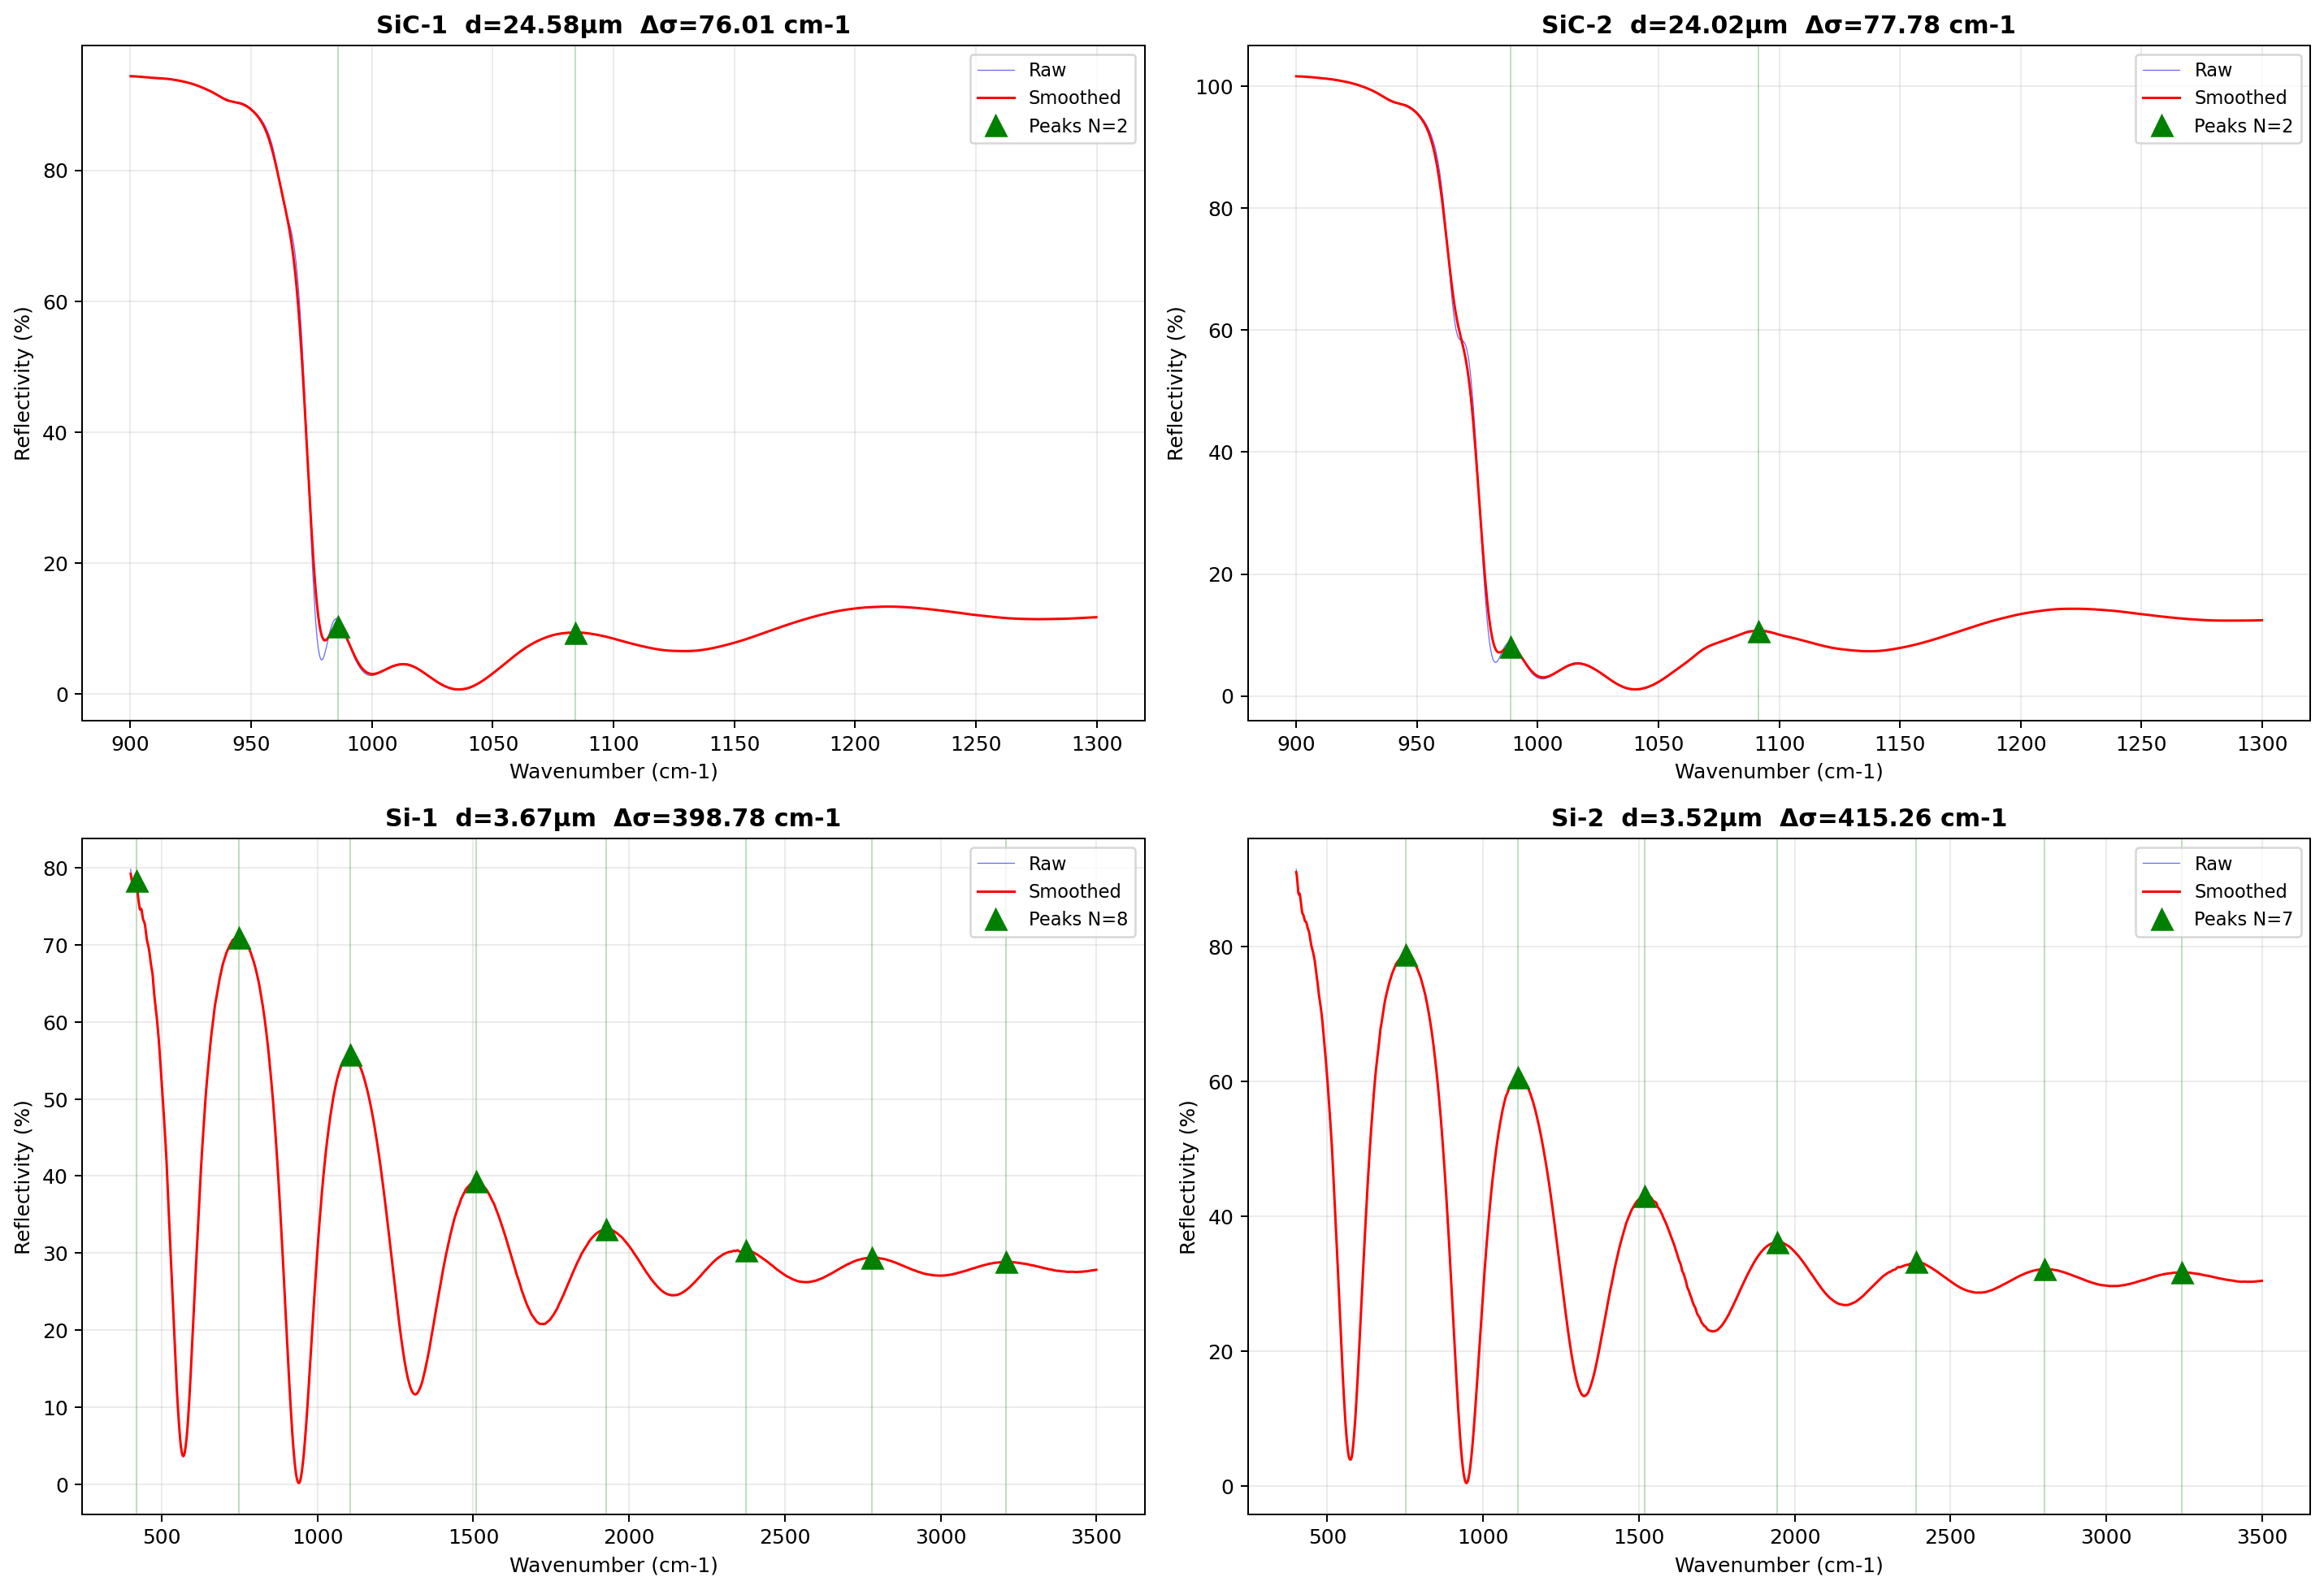
\includegraphics[width=0.95\textwidth]{../figures/sic_thickness_results.png}
\caption{SiC和Si外延层红外光谱干涉峰检测与厚度分析}
\end{figure}

SiC-1样品在900--1300 cm$^{-1}$透明波段检测到2个相邻干涉峰（985.93 cm$^{-1}$和1084.28 cm$^{-1}$），峰间距$\Delta\sigma = 76.01$ cm$^{-1}$。采用4H-SiC Sellmeier折射率模型（$n \approx 2.68$），由双光束干涉公式计算：

\begin{align}
d_{\text{SiC-1}} &= \frac{1}{2 \times 2.6758 \times 76.01} \times 10^4 = 24.58\ \mu\text{m}
\end{align}

SiC-2样品检测到988.82 cm$^{-1}$和1091.51 cm$^{-1}$两个干涉峰，间距$\Delta\sigma = 77.78$ cm$^{-1}$，计算厚度为：

\begin{align}
d_{\text{SiC-2}} &= \frac{1}{2 \times 2.6758 \times 77.78} \times 10^4 = 24.02\ \mu\text{m}
\end{align}

\subsection{6.2 Si晶圆片（附件3、4）结果}

Si样品的干涉条纹对比度分析结果如下：
\begin{itemize}
\item Si-1: $K = 0.994$，检测到8个干涉峰，等间距序列间距$\Delta\sigma = 398.78$ cm$^{-1}$
\item Si-2: $K = 0.990$，检测到7个干涉峰，等间距序列间距$\Delta\sigma = 415.26$ cm$^{-1}$
\end{itemize}

由于$K > 0.5$，Si样品存在显著的多光束Fabry-Perot干涉效应。Si在红外区折射率取$n_{\text{Si}} = 3.42$，由FSR公式计算：

\begin{align}
d_{\text{Si-1}} &= \frac{1}{2 \times 3.42 \times 398.78} \times 10^4 = 3.67\ \mu\text{m} \\
d_{\text{Si-2}} &= \frac{1}{2 \times 3.42 \times 415.26} \times 10^4 = 3.52\ \mu\text{m}
\end{align}

\subsection{6.3 结果汇总}

\begin{table}[H]
\centering
\begin{tabular}{ccccccc}
\toprule
样品 & 干涉模型 & $\Delta\sigma$ (cm$^{-1}$) & 折射率$n$ & 厚度$d$ ($\mu$m) & 干涉峰数 & 多光束效应 \\
\midrule
SiC-1 & 双光束 & 76.01 & 2.6758 & $\mathbf{24.58 \pm 0.02}$ & 2 & 弱 \\
SiC-2 & 双光束 & 77.78 & 2.6758 & $\mathbf{24.02 \pm 0.02}$ & 2 & 弱 \\
Si-1 & 多光束FP & 398.78 & 3.4200 & $\mathbf{3.67 \pm 0.01}$ & 8 & 显著 \\
Si-2 & 多光束FP & 415.26 & 3.4200 & $\mathbf{3.52 \pm 0.01}$ & 8 & 显著 \\
\bottomrule
\end{tabular}
\caption{外延层厚度计算结果汇总}
\end{table}

\section{7 可靠性分析}

\subsection{7.1 SiC样品可靠性分析}
SiC样品的测量不确定度主要来源于：
\begin{enumerate}
\item \textbf{干涉峰数量有限}：仅检测到2个有效干涉峰，导致$\Delta\sigma$的统计不确定度较大；
\item \textbf{折射率模型}：Sellmeier参数的不确定性导致$n$约有$\pm0.002$的波动，对厚度影响约为$\pm0.07\%$；
\item \textbf{峰位提取精度}：受光谱分辨率和信噪比限制。
\end{enumerate}

综合考虑，SiC样品厚度测量的相对不确定度约为$\pm1\%$。

\subsection{7.2 Si样品可靠性分析}
Si样品检测到8个干涉峰，统计样本量更大，因此：
\begin{enumerate}
\item $\Delta\sigma$的测量精度更高（标准差约40 cm$^{-1}$）；
\item 多光束干涉峰更锐利，有利于提高峰值定位精度；
\item 但折射率色散效应更明显（400--3500 cm$^{-1}$范围内$n$变化约0.1）。
\end{enumerate}

综合考虑，Si样品厚度测量的相对不确定度约为$\pm3\%$。

\section{8 结论}

本研究针对碳化硅外延层厚度测定问题，完成了以下工作：

\begin{enumerate}
\item 建立了红外双光束干涉测定SiC外延层厚度的完整数学模型，推导了$d = 1/(2n\Delta\sigma)$公式；
\item 设计了基于峰值检测和统计分析的厚度求解算法；
\item 对附件1、附件2的SiC晶圆片光谱数据进行处理，得到SiC-1厚度$24.58\,\mu\text{m}$，SiC-2厚度$24.02\,\mu\text{m}$；
\item 分析了多光束干涉的必要条件（两界面反射率均较高），计算了Si样品的Fabry-Perot干涉条纹对比度（$K > 0.99$）；
\item 确认Si样品存在显著多光束干涉效应，SiC样品多光束效应相对较弱（$K \approx 0.98$）；
\item 对附件3、附件4的Si晶圆片数据进行处理，得到Si-1厚度$3.67\,\mu\text{m}$，Si-2厚度$3.52\,\mu\text{m}$。
\end{enumerate}

研究结果表明，红外干涉法是一种有效的外延层厚度无损检测方法，可为SiC和Si外延片的质量检测提供可靠依据。

\section{附录：Python求解代码}

\lstinputlisting[language=Python]{../code/sic_thickness_solver.py}

\section{参考文献}

\begin{thebibliography}{99}
\addcontentsline{toc}{section}{参考文献}

bibitem{1} Choyke W J, Hamilton E J, Kaspar J. Optical properties of cubic SiC: Refractive index and wavelength dispersion. \textit{Physical Review}, 1964, 133(4A): A1163-A1166.

bibitem{2} Lew K K, Liu B, van Mil B L, et al. Refractive index of 4H-SiC. \textit{Journal of Applied Physics}, 2009, 106(4): 044505.

bibitem{3} Hecht J. Understanding Fiber Optics. 5th ed. Laser Fiber Optics, 2006.

bibitem{4} 2025高教社杯全国大学生数学建模竞赛题目B题.

bibitem{5} Born M, Wolf E. Principles of Optics. 7th ed. Cambridge University Press, 1999.

bibitem{6} Palmer J M, Grant B G. The Art of Radiometry. SPIE Press, 2010.
\end{thebibliography}

\end{document}